\part{Connection on a manifold}

\chapter{What is a connection?}

    The structure of a differentiable manifold does not present a notion of intrinsic parallelism between two vectors that live in different tangent spaces at different points. Although things are different at one point because two vectors that live in the same tangent space are parallel if they are linearly dependent, i.e.~proportional to each others, the only way to have parallel vectors along a given path is to introduce an external rule. This rule is called a \textit{parallel transport}. It is another prescription to compare vectors at different points, different from the push-forward.
    
\section{Covariant derivative}

    Suppose we have a parallel transport for a vector $W$ on a curve $\gamma$ tangent to a vector field $V = \dv{}{\lambda}$. If the vector $W \in T_{Q(\lambda)}$ is defined at a point $Q$ parametrised by $\lambda$, then we can associate a second vector $W^\parallel_{-\Delta \lambda} \in T_{P(\lambda_0)}$ at a different point $P$ parametrised by $\lambda_0$ such that $\lambda = \lambda_0 + \Delta \lambda$. By means of the parallel transport, we can move back the vector defined in $Q(\lambda)$ by a shift $-\Delta \lambda$ in order to make them comparable at the point $P(\lambda_0)$, which means that they are both in the same tangent space $T_{P(\lambda_0)}$. See Figure~\ref{fig:covder}.

    \begin{figure}[h!]
        \centering
        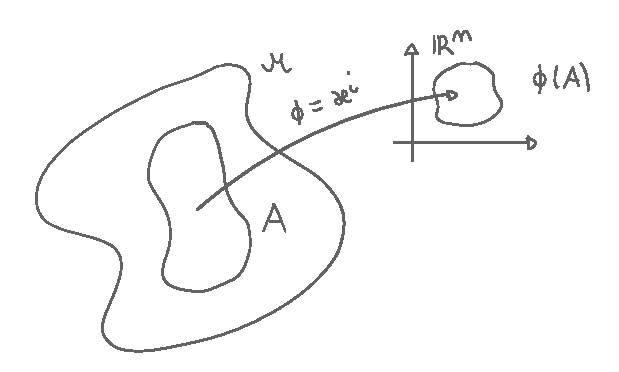
\includegraphics{chart.pdf}
        \caption{The parallel transport of a vector field $W$ along the vector $V$.}\label{fig:covder}
    \end{figure}

    \begin{definition}[Covariant derivative]
        The covariant derivative of a vector field $W$ with respect to $V=\dv{}{\lambda}$ at a point $P(\lambda_0)$ is 
        \begin{equation*}
            \nabla_V W \vert_{\lambda_0} = \lim_{\Delta \lambda \rightarrow 0} \frac{W^{\parallel}_{- \Delta \lambda} (\lambda_0) - W(\lambda_0)}{\Delta \lambda} ~.
        \end{equation*}
    \end{definition}
    \noindent It vanishes if the vector does not change along $\gamma$, the parallel transported vector coincides with the original one $W^{\parallel} = W$. It is different from the Lie derivative because we do not need an entire congruence so that the vectors are defined in a neighbourhood of the curve, we only need one curve and a parallel transport.

\subsection{Covariant derivative of functions and vectors}

    Since for a function there is no direction, the covariant derivative of a function is the same as the Lie derivative~\ref{liederf}
    \begin{equation*}
        \nabla_V f = \dv{f}{\lambda} ~.
    \end{equation*}
    For a generic vector, we require the following properties
    \begin{enumerate}
        \item Leibniz rules, i.e.~for a function and a vector
            \begin{equation}\label{covlei}
                \nabla_V (f W) = \dv{f}{\lambda} W + f \nabla_V W ~,
            \end{equation}
                for the tensor product of two vectors
            \begin{equation*}
                \nabla_V (A \otimes B) = A \otimes \nabla_V B + \nabla_V A \otimes B ~,
            \end{equation*}
                for the contraction of a $1$-form with a vector
            \begin{equation*}
                \nabla_V (\omega (A)) = (\nabla_V \omega) A + \omega (\nabla_V A) ~;
            \end{equation*}
        \item no effects on reparameterisation $\mu = \mu(\lambda)$, i.e. 
             \begin{equation}\label{covre}
                \nabla_{h V} W = h \nabla_V W ~,
            \end{equation}
            where $h = \dv{\mu}{\lambda}$ such that 
            \begin{equation*}
                \dv{}{\mu} = \dv{\lambda}{\mu} \dv{}{\lambda} = h \dv{}{\lambda} ~;
            \end{equation*}
        \item linearity, i.e.~the covariant derivative of two vectors at a point is additive
            \begin{equation*}
                \nabla_V A + \nabla_W A = \nabla_{V + W} A ~.
            \end{equation*} 
    \end{enumerate}
    The second property implies that for all smooth functions $h$, the notion of parallel transport along a curve must be independent on reparameterisation
    \begin{equation*}
        \nabla_V W = 0 \quad \Rightarrow \quad \nabla_{hV} W = 0 ~.
    \end{equation*}
    The second and the third property together imply that $\forall f, g$
    \begin{equation*}
        \nabla_{fV+gW} A = f \nabla_V + g \nabla_W ~.
    \end{equation*}
    The Lie derivative does not satisfy the second property. 
    \begin{proof}
        Infact
        \begin{equation*}
        \begin{aligned}
            \pounds_{hV} W & = [hV, W] \\ & = h [V, W] + [h, W] V \\ &= h [V, W] - [W, h] V \\ & = h \pounds_V W - (\pounds_W h) V \neq h \pounds_V W ~,
        \end{aligned}
        \end{equation*}
        where we have used~\eqref{leib} and~\eqref{anti}.
    \end{proof}

\section{Affine connection}

    In order to find the components of the covariant derivative, we expand on a basis $\{e_i\}$ of $T_{P(\lambda_0)}$ both $V = V^i e_i$ and $W = W^j e_j$
    \begin{equation}\label{covder1}
    \begin{aligned}
        \nabla_V W & = \nabla_{V^i e_i} (W^j e_j) \\ & = V^i \nabla_{e_i} (W^j e_j) \\ & = V^i (\nabla_{e_i} W^j) e_j + V^i W^j \nabla_{e_i} e_j \\ & = V^i (\nabla_{e_i} W^j) e_j + V^i W^j \Gamma^k_{ji} e_k ~,
    \end{aligned}
    \end{equation}
    where we have used~\eqref{covlei} and~\eqref{covre}. The second term is the \textit{affine connection}
    \begin{equation}\label{affconn}
        \nabla_{e_i} e_j = \Gamma^k_{ji} e_k ~.
    \end{equation} 
    It follows that the affine connection fixes the parallel transport: once we know all the $i-th$ and $j-th$ components, we know how to do it. Furthermore, it transforms like a tensor at fixed $i$ and $j$ but it is not a $(1,2)$ tensor, infact for a change of basis $e_{i'} = \Lambda_{i'}^{\phantom{i'} i} e_i$ it transforms as 
    \begin{equation*}
        \Gamma^{k'}_{j'i'} = \Lambda^{k}_{\phantom{k} k'}(\Lambda^{i}_{\phantom{i} i'} \Lambda^{j}_{\phantom{j} j'} \Gamma^k_{ji} + \Lambda^{i}_{\phantom{i} i'} \partial_i \Lambda^{k'}_{\phantom{k'} j'} ) ~,
    \end{equation*}
    which shows that only at fixed $i$ and $j$, it behaves as a tensor such that 
    \begin{equation*}
        \Gamma^{k'}_{ij} e_{k'} = \Gamma^k_{ij} e_k ~.
    \end{equation*}
    \begin{proof}
        Given a coordinate basis $\{e_i\}$ and a change of basis $e_{i'} = \Lambda^{i}_{\phantom{i} i'} e_i$
        \begin{equation*}
        \begin{aligned}
            \Gamma^{k'}_{j'i'} e_{k'} & = \nabla_{e_{i'}} e_{j'} \\ & = \nabla_{\Lambda^{i}_{\phantom{i} i'} e_i} (\Lambda^{j}_{\phantom{j} j'} e_j) \\ & = \Lambda^{i}_{\phantom{i} i'} \nabla_{e_i} (\Lambda^{j}_{\phantom{j} j'} e_j) \\ & = \Lambda^{i}_{\phantom{i} i'} \Lambda^{j}_{\phantom{j} j'}\nabla_{e_i} e_j + \Lambda^{i}_{\phantom{i} i'}  (\nabla_{e_i} \Lambda^{j}_{\phantom{j} j'}) e_j \\ & = \Lambda^{i}_{\phantom{i} i'} \Lambda^{j}_{\phantom{j} j'} \Gamma^k_{ji} e_k + \Lambda^{i}_{\phantom{i} i'} (\partial_i \Lambda^{j}_{\phantom{j} j'}) e_k \\ & = \Lambda^{i}_{\phantom{i} i'} \Lambda^{j}_{\phantom{j} j'} \Gamma^k_{ji} \Lambda^{k}_{\phantom{k} k'} e_{k'} + \Lambda^{i}_{\phantom{i} i'} (\partial_i \Lambda^{k'}_{\phantom{k'} j'}) \Lambda^{k}_{\phantom{k} k'} e_{k'} \\ & = \Lambda^{k}_{\phantom{k} k'}(\Lambda^{i}_{\phantom{i} i'} \Lambda^{j}_{\phantom{j} j'} \Gamma^k_{ji} + \Lambda^{i}_{\phantom{i} i'} \partial_i \Lambda^{k'}_{\phantom{k'} j'} ) e_{k'} 
        \end{aligned}
        \end{equation*}
        where we have used~\eqref{affconn},~\eqref{covlei},~\eqref{covre}, $e_{i} = \Lambda_{i}^{\phantom{i} i'} e_{i'}$ and $\nabla_{e_i} \Lambda_{i}^{\phantom{i} i'} = \partial_i \Lambda_{i}^{\phantom{i} i'}$, and we exchange $j \leftrightarrow k'$. Hence, hiding the $e_{k'}$
        \begin{equation*}
            \Gamma^{k'}_{j'i'} = \Lambda^{k}_{\phantom{k} k'}(\Lambda^{i}_{\phantom{i} i'} \Lambda^{j}_{\phantom{j} j'} \Gamma^k_{ji} + \Lambda^{i}_{\phantom{i} i'} \partial_i \Lambda^{k'}_{\phantom{k'} j'} ) ~.
        \end{equation*}
    \end{proof}

    Once the $\Gamma$'s are given, we can find the components of the covariant derivative 
    \begin{equation}\label{covder}
        (\nabla W^k)_i = \partial_i W^k + \Gamma^k_{ji} W^j ~,
    \end{equation}
    or, equivalently, in different notation
    \begin{equation*}
        \nabla_i W^k = W^k_{;i} = W^k_{,i} + \Gamma^k_{ji} W^j ~.
    \end{equation*}
    Intuitively, the affine connection tells you what to mix in order to keep parallelism.
    \begin{proof}
        Infact, using~\eqref{covder1}
        \begin{equation*}
        \begin{aligned}
            \nabla_V W & = V^i (\nabla_{e_i} W^j) e_j + V^i W^j \Gamma^k_{ji} e_k \\ & = V^i (\partial_i W^j) \pdv{}{x^j} + V^i W^j \Gamma^k_{ji} \pdv{}{x^k} \\ & = V^i (\partial_i W^k + V^i W^j \Gamma^k_{ji}) \pdv{}{x^k} ~,
        \end{aligned}
        \end{equation*}
        where we have exchanged $j \leftrightarrow k$. Hence, the $k$-th component is
        \begin{equation*}
            (\nabla_V W)^k = V^i \partial_i W^k + \Gamma^k_{ji} V^i W^j ~,
        \end{equation*}
        and since the components of $V$ enter only by contraction in a multiplicative way, we obtain
        \begin{equation*}
            (\nabla W^k)_i = \partial_i W^k + \Gamma^k_{ji} W^j ~.
        \end{equation*}
    \end{proof}

\subsection{Covariant derivative of 1-forms and generic tensors}

    The covariant derivative of a $1$-form is 
    \begin{equation*}
        \omega_{k;i} = \nabla_i \omega_k = \partial_i \omega_k - \Gamma^j_{ki} \omega_j ~.
    \end{equation*}
    \begin{proof}
        By contraction, $\omega (V) = \omega_i V^k$ is a scalar and using~\eqref{covlei}
        \begin{equation*}
            \nabla_i (\omega_k V^k) = (\nabla_i \omega_k) V^k + \omega_k (\nabla_i V^k) ~,
        \end{equation*}
        and, since for a scalar partial and covariant derivative are equivalent 
        \begin{equation*}
            \nabla_i (\omega_k V^k) = \partial (\omega_k V^k) = (\partial_i \omega_k) V^k + \omega_k (\partial_i V^k) ~.
        \end{equation*}
        Hence, using~\eqref{covder}
        \begin{equation*}
        \begin{aligned}
            (\partial_i \omega_k) V^k + \cancel{\omega_k (\partial_i V^k)} & = (\nabla_i \omega_k) V^k + \omega_k (\nabla_i V^k) \\ & = (\nabla_i \omega_k) V^k + \omega_k (\partial_i V^k + \Gamma^k_{ij} V^j) \\ & = (\nabla_i \omega_k) V^k + \cancel{\omega_k \partial_i V^k} + \omega_k \Gamma^k_{ij} V^j~,
        \end{aligned}
        \end{equation*}
        and isolating the covariant derivative of a 1-form 
        \begin{equation*}
            (\nabla_i \omega_k) V^k = (\partial_i \omega_k) V^k - \omega_j \Gamma^k_{ik} V^k ~.
        \end{equation*}
    \end{proof}
    The covariant derivative of a $(1,1)$ tensor is 
    \begin{equation*}
        T^i_{\phantom i j;k} = T^i_{\phantom i j,k} + \Gamma^i_{lk} T^l_{\phantom l j} - \Gamma^l_{jk} T^i_{\phantom i l} ~.
    \end{equation*}
    \begin{proof}
        By contraction, $T (\omega, V) = T^i_{\phantom i j} \omega_i V^j$ is a scalar and using~\eqref{covlei}
        \begin{equation*}
            \nabla_k (T^i_{\phantom i j} \omega_i V^j)  = (\nabla_k T^i_{\phantom i j}) \omega_i V^j + T^i_{\phantom i j} (\nabla_k \omega_i) V^j + T^i_{\phantom i j} \omega_i  (\nabla_k V^j) ~,
        \end{equation*}
        and, since for a scalar partial and covariant derivative are equivalent 
        \begin{equation*}
            \nabla_k (T^i_{\phantom i j} \omega_i V^j) = \partial_k (T^i_{\phantom i j} \omega_i V^j) = (\partial_k T^i_{\phantom i j}) \omega_i V^j + T^i_{\phantom i j} (\partial_k \omega_i) V^j + T^i_{\phantom i j} \omega_i  (\partial_k V^j) ~.
        \end{equation*}
        Hence, using~\eqref{covder}
        \begin{equation*}
        \begin{aligned}
            (\partial_k T^i_{\phantom i j}) \omega_i V^j & + \cancel{T^i_{\phantom i j} (\partial_k \omega_i) V^j} + \cancel{T^i_{\phantom i j} \omega_i (\partial_k V^j)} = (\nabla_k T^i_{\phantom i j}) \omega_i V^j + T^i_{\phantom i j} (\nabla_k \omega_i) V^j + T^i_{\phantom i j} \omega_i  (\nabla_k V^j) \\ & = (\nabla_k T^i_{\phantom i j}) \omega_i V^j + T^i_{\phantom i j} (\partial_k \omega_i - \Gamma^l_{ik} \omega_l) V^j + T^i_{\phantom i j} \omega_i (\partial_k V^j + \Gamma^j_{lk} V^l) \\ & = (\nabla_k T^i_{\phantom i j}) \omega_i V^j + \cancel{T^i_{\phantom i j} (\partial_k \omega_i) V^j} - T^i_{\phantom i j}  \Gamma^l_{ik} \omega_l V^j + \cancel{T^i_{\phantom i j} \omega_i (\partial_k V^j)} + T^i_{\phantom i j} \omega_i \Gamma^j_{lk} V^l ~,
        \end{aligned}
        \end{equation*}
        and isolating the covariant derivative of a 1-form 
        \begin{equation*}
            (\nabla_k T^i_{\phantom i j}) \omega_i V^j = (\partial_k T^i_{\phantom i j}) \omega_i V^j + \Gamma^i_{lk} T^l_{\phantom l j} \omega_i V^j - \Gamma^l_{jk} T^l_{\phantom i l} \omega_i  V^j ~,
        \end{equation*}
        where we exchanged $i \leftrightarrow l$ in the second term and $j \leftrightarrow l$ in the last one.
    \end{proof}
    The covariant derivative of a generic $(n,m)$ tensor is 
    \begin{equation*}
        T^{i \ldots n}_{\phantom{i \ldots n} j \ldots m; k} = T^{i \ldots n}_{\phantom{i \ldots n} j \ldots m, k} + \Gamma^i_{lk} T^{l \ldots n}_{\phantom{i \ldots n} j \ldots m} + \ldots + \Gamma^n_{lk} T^{i \ldots l}_{\phantom{i \ldots n} j \ldots m} - \Gamma^l_{jk} T^{i \ldots n}_{\phantom{i \ldots n} l \ldots m} - \ldots - \Gamma^l_{mk} T^{i \ldots n}_{\phantom{i \ldots n} j \ldots l}~.
    \end{equation*}

\subsection{Symmetric connection and torsion}

    An affine connection is symmetric if 
    \begin{equation}\label{symm}
        \Gamma^k_{ij} = \Gamma^k_{ji}  ~,
    \end{equation}
    and it implies the relation with the Lie derivative
    \begin{equation*}
        \nabla_V W - \nabla_W V = [V, W] = \pounds_V W ~.
    \end{equation*}
    \begin{proof}
        Infact, using~\eqref{covder1} and~\eqref{symm}
        \begin{equation*}
        \begin{aligned}
            \nabla_V W - \nabla_W V & = V^i (\nabla_{e_i} W^j) e_j + V^i W^j \Gamma^k_{ji} e_k - W^i (\nabla_{e_i} V^j) e_j - W^i V^j \Gamma^k_{ji} e_k \\ & = V^i (\nabla_{e_i} W^j) e_j + V^i W^j \Gamma^k_{ji} e_k - W^i (\nabla_{e_i} V^j) e_j - W^j V^i \Gamma^k_{ij} e_k \\ & = V^i (\nabla_{e_i} W^j) e_j + \cancel{V^i W^j \Gamma^k_{ji} e_k} - W^i (\nabla_{e_i} V^j) e_j - \cancel{W^j V^i \Gamma^k_{ji} e_k} \\ & = V^i (\nabla_{e_i} W^j) e_j - W^i (\nabla_{e_i} V^j) e_j \\ & = [V, W] = \pounds_V W ~,
        \end{aligned}
        \end{equation*}
        where we have exchanged $i \leftrightarrow j$ and~\eqref{liecomp}.
    \end{proof}

    Geometrically, it means that two linearly independent vectors $V$ and $W$ at a point $P$, which are parallel transported along the other ($W^\parallel$ along $V$ and $V^\parallel$ along $W$) forms a closed path. Infact, since $\nabla_V W^\parallel = \nabla_W V^\parallel = 0$, it follows that $\pounds_{V^\parallel} W^\parallel = [V^\parallel, W^\parallel] = 0$ and, in a coordinate frame, if we move along $V$ and $W^\parallel$ or along $W$ and $V^\parallel$, we end up in the same point. On the other hand, if the affine connection is not symmetric, it is subjected to torsion 
    \begin{equation*}
        T^k_{ji} = \Gamma^k_{ij} - \Gamma^k_{ji} \neq 0 ~,
    \end{equation*}
    which means that the close path does not close. See Figure~\ref{fig:tors}.

    \begin{figure}[h!]
        \centering
        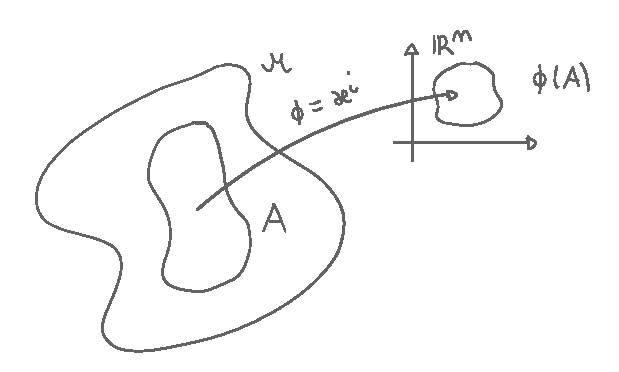
\includegraphics{chart.pdf}
        \caption{On the left, a symmetric connection means that the path does closed. On the right, torsion means that the path does not close.}\label{fig:tors}
    \end{figure}

\section{Geodesics}

    \begin{definition}[Geodesics]
        A curve $\gamma$ tangent to a vector $V$ is a geodesics if 
        \begin{equation*}
            \nabla_V V \vert_P = 0 \quad \forall P \in \gamma
        \end{equation*}
        where $\lambda$ is called an affine parameter. 
    \end{definition}

    The definition is restricted because we could have simply request 
    \begin{equation*}
        \nabla_V V = \alpha V
    \end{equation*}
    where $\alpha$ is a real function. It is invariant under reparameterization of the curve 
    \begin{equation*}
        \nabla_{h V} V = h \nabla_V V = h \alpha V = \alpha' V
    \end{equation*}

    Given a coordinate frame 
    \begin{equation*}
        0 = (\nabla_V V)^k = V^j \Big( \pdv{V^k}{x^j} + \Gamma^k_{ij} V^i \Big) = \dv{V^k}{\lambda} + \Gamma^k_{ij} V^i V^j = \dvd{x^k}{\lambda} + \Gamma^k_{ij} \dv{x^i}{\lambda} \dv{x^j}{\lambda}
    \end{equation*}
    which is a system of $n$ second-order ordinary differential equations. 

    With the geodesics, we can use the affine parameter as coordinate $x^1 = \lambda$. The corresponding basis vector
    \begin{equation*}
        \nabla_{e_1} e_1 = 0
    \end{equation*}
    and the remaining ones can be parallely transported, which give rise to adapted coordinates 
    \begin{equation*}
        0 = \nabla_{e_1} e_i = \Gamma^k_{i1} e_k
    \end{equation*}
    Hence 
    \begin{equation*}
        \Gamma^k_{i1}(P) = 0 \quad \forall i,k = 1, \ldots n \quad \forall P \in \gamma
    \end{equation*}
    However, in general $\Gamma^k_{ij} \neq 0$ for $j \neq 1$.

    At a point $P$, for ant basis, the $n$ geodesic equations 
    \begin{equation*}
        \nabla_{e_i} e_i = 0
    \end{equation*}
    admit a unique solution with initial condition $e_i(P) = e_i^{(0)}$, which defines $n$ coordinates $\lambda_{(i)} = x^i$. Hence, the affine connection vanishes at $P$ for any geodesics 
    \begin{equation*}
        \Gamma^k_{ij} \vert_P = 0
    \end{equation*}
    and the system is called normal or Gaussian frame.

    The affine connection defines how coordinate basis vectors are parallelly transported. Infact
    \begin{equation*}
        (\nabla_V W)^j \vert_P = V^i \pdv{W^j}{x^i} \Big \vert_P
    \end{equation*}
    then $W$ is parallely tranported along $V$ if its components do not change. In such frame 
    \begin{equation*}
        \nabla_{e_i} \vert_P = \pdv{}{x^i} \Big \vert_P = \pounds_{e_i} \vert_P
    \end{equation*}
    and the covariant derivatives coincides with the Lie derivatives. However, for another point $Q \neq P$, this does not hold, because in general it is impossible to find an open set such that 
    \begin{equation*}
        \pdv{\Gamma^k_{ij}}{x^l} \Big \vert_P = \Gamma^k_{ij,l} \vert_P \neq 0 
    \end{equation*}
    and higher derivatives. It is possible to construct a normal frame in an open set of $P$ along the geodesics.

    Given a vector $A_P$ at a point $P = \gamma(\lambda_0)$ along $V = \dv{}{\lambda}$ and another point $Q = \gamma(\lambda = \lambda_0 + \Delta \lambda)$ 
    \begin{equation*}
        A(Q) = A_P + \Delta \lambda \nabla_V A_P + \frac{1}{2} \Delta \lambda^2 \nabla_V \nabla_V A_P + \ldots = \exp(\Delta \lambda \nabla_V) A_P
    \end{equation*}
    and, introducing a basis vector, 
    \begin{equation*}
        0 = \nabla_V e_i \vert_\gamma = V^j \Gamma^k_{ji} e_k \vert_\gamma 
    \end{equation*}
    which implies that the geodesic map becomes the exponential map along $\gamma$ 
    \begin{equation*}
        A^i(Q) = \exp(\Delta \lambda V^j \partial_j) A^i_P = A^i_P + \Delta \lambda V^j \partial_j A^i_P + O(\Delta \lambda^2) = A^i_P
    \end{equation*}
    Hence, the exponential map defines a vector field $A$ mapping it along $V$. Since the components do not change, all the vector $A(\lambda)$ are parallel to $A_P$.

    In a generic frame, we substitute partial derivatives with covariant derivatives
    \begin{equation*}
        A(Q) = A^i_P \Delta \lambda V^j \Gamma^i_{jk} A^k_P + O(\Delta \lambda^2) 
    \end{equation*}
    If $A = V$, it defines the geodesic curve itself.

\chapter{Riemmann tensor}

    \begin{definition}[Riemann tensor]
        The Riemann tensor is a $(1,3)$ tensor defined as 
        \begin{equation*}
            R(V,W) A = [\nabla_V, \nabla_W] A - \nabla_{[V,W]} A
        \end{equation*}
        or in components 
        \begin{equation*}
            R(V, W) A = (R(V,W)^i_{\phantom i j} A^j) e_i
        \end{equation*}
    \end{definition}

    Through the Riemann tensor, we could define the curvature of a manifold.

    Geometrically, consider two commuting vector fields $V = \dv{}{\lambda}$ and $W = \dv{}{\mu}$, used to construct a closed path. Consider a third vector $A$, start from a point $P$ and move it, first along $V$ by $\delta \lambda$ and then along $W$ by $\delta \mu$
    \begin{equation*}
        A^\parallel_{WV} = \exp(\delta \mu \nabla_W) \exp(\delta \lambda \nabla_V) A
    \end{equation*}
    or the other way 
    \begin{equation*}
        A^\parallel_{VW} = \exp(\delta \lambda \nabla_V) \exp(\delta \mu \nabla_W)  A
    \end{equation*}

    For infinitesimal displacement, the difference between the two path is 
    \begin{equation*}
        \delta A = A^\parallel_{WV} - A^\parallel_{VW} = \delta \mu \delta \mu [\nabla_V, \nabla_W] A + O(\delta^3)
    \end{equation*}
    Using the Riemann tensor 
    \begin{equation*}
        \delta A = \delta \mu \delta \mu R(V,W) A + O(\delta^3)
    \end{equation*}
    or introducing the second derivative 
    \begin{equation*}
        \frac{\delta^2 A^i}{\delta \mu \delta \lambda} = R^i_{jkl} V^j W^k A^l + O(\delta^3)
    \end{equation*}

    Hence, if the Riemann tensor vanishes, a vector parallely transported along a closed path does not return back to its initial value, otherwise, the manifold is curved. It is an intrinsic curvature because it does not need the embedding in a higher dimensional space. 

    The Riemann tensor has the following way 
    \begin{enumerate}
        \item scalar, i.e. 
            \begin{equation*}
                R(V,W) (fA) = f R(V, W) A
            \end{equation*}
        \item scalar, i.e. 
            \begin{equation*}
                R(fV,W) A = R(V, fW) A = f R(V, W) A
            \end{equation*}
        \item in coordinates, i.e. 
            \begin{equation*}
                R^i_{ljk} e^l \otimes e_i = R(e_j, e_k)^i_l e^l \otimes e_i
            \end{equation*}
    \end{enumerate}

\section{Metric connection}

    In a metric manifold, we are interested in parallel transport which preserves lengths and angles. Consider two vectors $A$ and $B$ parallely transported along $V$, i.e. $\nabla_V A = \nabla_V B = 0$. We request that 
    \begin{equation*}
        \nabla_V g(A,B) = 0
    \end{equation*}
    which implies
    \begin{equation*}
        \nabla_V g = 0
    \end{equation*}
    or 
    \begin{equation}\label{metconn}
        \nabla g = 0
    \end{equation}

    This implies that the affine connection is fixed by the metric 
    \begin{equation}\label{chr}
        \Gamma^k_{ij} = \frac{1}{2} g^{kl} (g_{il,j} + g_{jl,i} - g_{ij,l})
    \end{equation}
    where $\Gamma^k_{ij}$ are called Christoffel symbols.

    \begin{proof}
        The components of the covariant derivative are 
        \begin{equation*}
            0 = g_{ij;l} = g_{ij,l} - \Gamma^a_{il} g_{aj} - \Gamma^a_{jl} g_{ia}
        \end{equation*}
        and, permutating the indices
        \begin{equation*}
            0 = g_{il;j} = g_{il,j} - \Gamma^a_{ij} g_{al} - \Gamma^a_{lj} g_{ia}
        \end{equation*}
        \begin{equation*}
            0 = g_{jl;i} = g_{jl,i} - \Gamma^a_{ji} g_{al} - \Gamma^a_{li} g_{ja}
        \end{equation*}

        Hence, contracting with the inverse of the metric
        \begin{equation*}
        \begin{aligned}
            g^{kl} (g_{il,j} + g_{jl,i} - g_{ij,l}) & = \Gamma^k_{ij} + g^{kl} \Gamma^a_{lj} g_{ia} + \Gamma^k_{ji} + g^{kl} \Gamma^a_{li} g_{ja} - g^{kl} \Gamma^a_{il} g_{aj} - g^{kl} \Gamma^a_{jl} g_{ia} \\ & = \Gamma^k_{ij} + \Gamma^k_{ji} + g^{kl} (\Gamma^a_{li} - \Gamma^a_{il}) g_{ja} + g^{kl} (\Gamma^a_{lj} - \Gamma^a_{jl}) g_{ia}
        \end{aligned}
        \end{equation*}

        The symmetry of $g$ implies the symmetry of $\Gamma^k_{ij} = \Gamma^k_{ji}$.

        Furthermore, the metric fixes the Christoffel symbols 
        \begin{equation*}
            \Gamma^k_{ij} = \frac{1}{2} g^{kl} (g_{il,j} + g_{jl,i} - g_{ij,l})
        \end{equation*}
    \end{proof}

    If the metric is in canonical form at $P$, the Christoffel symbols become 
    \begin{equation*}
        \Gamma^k_{ij} \vert_P = 0
    \end{equation*}

    Geodetics are local extremal length. Consider a geodesic $\gamma$ and a normal frame around it. In a neighbourhood of $\gamma$, the metric is in canonical form and the length becomes 
    \begin{equation*}
        ds^2 \simeq \frac{1}{2} \pdvdu{g_{ii}}{(\eta^i)} \Big \vert_{\lambda_P, \eta^1=\ldots=\eta^{n-1}=0}
    \end{equation*}
    This means that each portion of the geodesic is a local extremum (minimum if the second derivative is positive, maximum if negative).~\eqref{chr} can be derived from that.

    \begin{proof}
        The length of a curve between two fixed end-points is 
        \begin{equation*}
            s = \int_{A}^{B} ds = \int_{A}^{B} ds \sqrt{g_{ij} \dot x^i \dot x^j} = \int_{\lambda_A}^{\lambda_B} d\lambda \sqrt{2 L(x^k, \dot x^l)}
        \end{equation*}
        If we define $\lambda = s$, then $2L = 1$. A variation of the length is 
        \begin{equation*}
            \delta s = \delta \int_{s_A}^{s_B} ds \sqrt{2L} = \int_{s_A}^{s_B} ds \frac{\delta L}{\sqrt{2L}} = \delta \int_{s_A}^{s_B} ds L(x^k, \dot x^l)
        \end{equation*}

        Hence, if the variation vanishes, we have the Euler-Lagrange equations 
        \begin{equation*}
            \dv{}{s} \pdv{L}{\dot x^m} - \pdv{L}{x^m} = 0
        \end{equation*}

        In particular, 
        \begin{equation*}
            \pdv{L}{x^m} = \frac{1}{2} g_{jk,m} \dot x^j \dot x^k
        \end{equation*}
        \begin{equation*}
            \pdv{L}{\dot x^m} = g_{mj} \dot x^j
        \end{equation*}
        and the Euler-Lagrange equations are 
        \begin{equation*}
            \ddot x^i + \frac{1}{2} g^{il} (g_{lk,j} + g_{lj,k} - g_{jk,l}) \dot x^j \dot x^k = 0
        \end{equation*}
        which, compared to the geodesic equation 
        \begin{equation*}
            \ddot x^i + \Gamma^i_{jk} \dot x^j \dot x^k = 0
        \end{equation*}
        gives the result.
    \end{proof}

    Consider a geodesic $\gamma_1$ from a point $P_1$ with two orthogonal tangent vectors $V_1 = \dv{}{\lambda}$ and $Y = \dv{}{y}$ such that $g(V_1,V_1) = -1$, $g(Y, Y) > 0$, $g(V_1, Y) = 0$. Moving from $P_1$ by $\Delta y$ at $P_2$ from which starts a geodesic $\gamma_2$ tangent to $V_2$ such that $\nabla_Y V_2 = 0$. Parametrising by $\lambda$ the two geodesic. If the manifold is flat, the length of $Y$ is constant and $\Delta y$ is equal to the distance between $\gamma_1(\lambda)$ and $\gamma_2(\lambda)$. Otherwise, if the manifold is curved, the rate of change of this distance is 
    \begin{equation*}
        \ddot Y^i \simeq \dvf{V^i}{\lambda^2} \simeq R^i_{jkl} V^j Y^k V^l
    \end{equation*}

\section{Killing equation}

    The Killing equation~\eqref{kill} in terms of the covariant derivative becomes 
    \begin{equation*}
        V_{i;j} + V_{j;i} = V_{(i,j)} = 0 ~.
    \end{equation*}

    \begin{proof}
        By contraction, $g(A,B)$ is a scalar
        \begin{equation*}
            \pounds_V g(A, B) = \nabla_V g(A,B) ~,
        \end{equation*}
        and using Leibniz rule, in a metric connection~\eqref{metconn}
        \begin{equation*}
        \begin{aligned}
            (\pounds_V g) (A, B) + g(\pounds_V A, B) + g(A, \pounds_V B) & = \underbrace{(\nabla_V g)}_0 (A, B) + g(\nabla_V A, B) + g(A, \nabla_V B) \\ & = g(\nabla_V A, B) + g(A, \nabla_V B) ~.
        \end{aligned}
        \end{equation*}
        We isolate the first term and we use coordinate basis, expanding $V = V^k e_k$
        \begin{equation*}
        \begin{aligned}
            (\pounds_V g) (e_i, e_j) & = (\pounds_V g)_{ij} = - g(\pounds_V e_i, e_j) - g(e_i, \pounds_V e_j) + g(\nabla_V e_i, e_j) + g(e_i, \nabla_V e_j) \\ & = - g(\pounds_V e_i, e_j) - g(e_i, \pounds_V e_j) + V^k g(\nabla_{e_k} e_i, e_j) + V^k g(e_i, \nabla_{e_k} e_j) \\ & = \partial_i V^k g(e_k, e_j) + \partial_j V^k (e_i, e_k) + V^k \Gamma^l_{ik} g(e_l, e_j) + V^k \Gamma^l_{jk} g(e_i, e_l) \\ & (\partial_i V^k g_{kj} + V^k \Gamma^l_{ik} g_{lj}) + (\partial_j V^k g_{ki} + V^k \Gamma^l_{jk} g_{li}) \\ & = V_{j;i} + V_{i;j} ~,
        \end{aligned}
        \end{equation*}
        which vanishes by the Killing equation.
    \end{proof}

    In a normal frame at a point, where $\Gamma \vert_P = 0$, the Killing equation becomes 
    \begin{equation*}
        V_{(i,j)} \vert_P = 0 ~.
    \end{equation*}
    However, we need to define the Killing equation in at least an open set of the manifold if not in the entire of it.

\chapter{Ricci tensor, Ricci scalar, Einstein tensor}

    In a normal frame at a point, the Riemann tensor becomes 
    \begin{equation*}
        R_{ijkl} = \frac{1}{2} (g_{il,jk} - g_{ik,jl} + g_{jk,il} - g_{jl,ik}) ~.
    \end{equation*}
    It satisfies the following properties 
    \begin{enumerate}
        \item antisymmetry in the first and last pair of indices, i.e. 
        \begin{equation}\label{rieanti}
            R_{ijkl} = - R_{jikl} = - R_{ijlk} ~,
        \end{equation}
        \item block symmetry for the exchange of two pairs, i.e.
        \begin{equation}\label{riesymm}
            R_{ijkl} = R_{klij} ~,
        \end{equation}
        \item first Bianchi identity, i.e. 
        \begin{equation}\label{bianchi1}
            R_{i jkl} + R_{i klj} + R_{i ljk} = 0 ~,
        \end{equation}
        \item second or contracted Bianchi identity, i.e. 
        \begin{equation}\label{bianchi2}
            R_{ijkl,m} + R_{ijmk,l} + R_{ijlm,k} = 0 ~.
        \end{equation}
    \end{enumerate}
    \begin{proof}
        For the antisymmetry property
        \begin{equation*}
        \begin{aligned}
            R_{ijkl} & = \frac{1}{2} (g_{il,jk} - g_{ik,jl} + g_{jk,il} - g_{jl,ik}) \\ & = - \frac{1}{2} (- g_{il,jk} + g_{ik,jl} - g_{jk,il} + g_{jl,ik}) \\ & = - \frac{1}{2} (g_{jl,ik} - g_{jk,il} + g_{ik,jl} - g_{il,jk}) = - R_{jikl} ~,
        \end{aligned}
        \end{equation*}
        and 
        \begin{equation*}
        \begin{aligned}
            R_{ijkl} & = \frac{1}{2} (g_{il,jk} - g_{ik,jl} + g_{jk,il} - g_{jl,ik}) \\ & = - \frac{1}{2} (- g_{il,jk} + g_{ik,jl} - g_{jk,il} + g_{jl,ik}) \\ & = - \frac{1}{2} ( g_{ik,jl} - g_{il,jk} + g_{jl,ik}  - g_{jk,il}) = - R_{ijlk} ~.
        \end{aligned}
        \end{equation*}

        For the block symmetry
        \begin{equation*}
        \begin{aligned}
            R_{ijkl} = \frac{1}{2} (g_{il,jk} - g_{ik,jl} + g_{jk,il} - g_{jl,ik}) = \frac{1}{2} (g_{jk,il} - g_{jl,ik} +  g_{il,jk} - g_{ik,jl}) = R_{jilk} ~.
        \end{aligned}
        \end{equation*}

        For the first Bianchi identity 
        \begin{equation*}
        \begin{aligned}
            R_{ijkl} + R_{iklj} + R_{iljk} & = \frac{1}{2} (g_{il,jk} - g_{ik,jl} + g_{jk,il} - g_{jl,ik} + g_{ij,kl} - g_{il,kj} \\ & \quad + g_{kl,ij} - g_{kj,il} + g_{ik,lj} - g_{ij,lk} + g_{lj,ik} - g_{lk,ij} ) \\ & = \frac{1}{2} (\cancel{g_{il,jk}} - \cancel{g_{ik,jl}} + \cancel{g_{jk,il}} - \cancel{g_{jl,ik}} + \cancel{g_{ij,kl}} - \cancel{g_{il,jk}} \\ & \quad + \cancel{g_{kl,ij}} - \cancel{g_{jk,il} } + \cancel{g_{ik,jl}} - \cancel{g_{ij,kl}} + \cancel{g_{jl,ik}} - \cancel{g_{kl,ij}}) = 0 ~,
        \end{aligned}
        \end{equation*}
        where we have used the fact that second partial derivatives commute and the metric tensor is symmetric.

        For the contracted Bianchi identity 
        \begin{equation*}
        \begin{aligned}
            R_{ijkl,m} + R_{ijmk,l} + R_{ijlm,k} & = \frac{1}{2} (g_{il,jkm} - g_{ik,jlm} + g_{jk,ilm} - g_{jl,ikm} + g_{ik,jml} - g_{im,jkl} \\ & \quad + g_{jm,ikl} - g_{jk,iml} + g_{im,jlk} - g_{il,jmk} + g_{jl,imk} - g_{jm,ilk} ) \\ & = \frac{1}{2} (\cancel{g_{il,jkm}} - \cancel{g_{ik,jlm}} + \cancel{g_{jk,ilm}} - \cancel{g_{jl,ikm}} + \cancel{g_{ik,jlm}} - \cancel{g_{im,jkl}} \\ & \quad + \cancel{g_{jm,ikl}} - \cancel{g_{jk,ilm}} +\cancel{g_{im,jkl}} - \cancel{g_{il,jkm}} + \cancel{g_{jl,ikm}} - \cancel{g_{jm,ikl}}) = 0 ~,
        \end{aligned}
        \end{equation*}
        where we have used the fact that second partial derivatives commute and the metric tensor is symmetric.
    \end{proof}
    In a generic frame, the Riemann tensor can be obtained by substituting the partial derivative with the covariant derivative 
    \begin{equation}\label{riemanmetric}
        R_{ijkl} = \frac{1}{2} (g_{il;jk} - g_{ik;jl} + g_{jk;il} - g_{jl;ik}) ~.
    \end{equation}
    The Riemann tensor in terms of the connection is 
    \begin{equation}\label{rieconn}
        R^i_{\phantom i jkl} = \Gamma^i_{jl,k} - \Gamma^i_{jk,l} + \Gamma^a_{jl} \Gamma^i_{ak} - \Gamma^a_{jk} \Gamma^i_{al}
    \end{equation}
    \begin{proof}
        Maybe in the future.
    \end{proof}
    The number of indipendent components of a Riemann tensor is 
    \begin{equation*}
        \frac{n^2 (n^2 - 1)}{12}
    \end{equation*}
    \begin{proof}
        A symmetric matrix has $\frac{n(n+1)}{2}$ degrees of freedom, while an antysymmetric matrix has $\frac{n(n-1)}{2}$ of them. Therefore, by~\eqref{rieanti} and~\eqref{riesymm}, the indipendent components are 
        \begin{equation*}
        \begin{aligned}
            \frac{1}{2} \Big ( \frac{n(n-1)}{2} \Big) \Big ( \frac{n(n-1)}{2} + 1 \Big) & = \frac{(n^2 - n) (n^2 - n + 1)}{8} \\ & = \frac{(n^4 - n^3 + n^2 - n^3 + n - n) }{8} \\ & = \frac{n^4 - 2n^3 + 3n^2 - 2n}{8} ~.
        \end{aligned}
        \end{equation*}
        Adding the further property~\eqref{bianchi1}, which is a totally antysimmetric tensor with $\frac{n(n-1)(n-2)(n-3)}{4!}$, we obtain
        \begin{equation*}
        \begin{aligned}
            \frac{n^4 - 2n^3 + 3n^2 - 2n}{8} - \frac{n(n-1)(n-2)(n-3)}{4!} & =  \frac{n^4 - 2n^3 + 3n^2 - 2n}{8} - \frac{ (n^2 - n) (n^2 - 5n + 6)}{24} \\ & = \frac{3n^4 - 6n^3 + 9n^2 - 6n}{24} - \frac{ n^4 - 5 n^3 + 6n^2 - n^3 + 5 n^2 + 6n}{24} \\ & = \frac{2 n^4 - 2n^2}{24} = \frac{n^2 (n^2 - 1)}{12} ~. 
        \end{aligned}
        \end{equation*}
    \end{proof}

    In particular, we can define three new tensors by the block property: 
    \begin{enumerate}
        \item Ricci tensor, i.e. 
            \begin{equation}\label{riccit}
                R_{ij} = R^k_{\phantom k ikj} ~,
            \end{equation}
            such that $R_{ij} = R_{ji}$,
        \item Ricci scalar, i.e. 
            \begin{equation}\label{riccis}
                R = R^k_{\phantom k k} ~,
            \end{equation}
        \item Einstein tensor, i.e. 
            \begin{equation}\label{einstens}
                G_{ij} = R_{ij} - \frac{1}{2} R g_{ij} ~.
            \end{equation}
    \end{enumerate}
    The Ricci tensor in terms of the connection is 
    \begin{equation*}
        R_{ij} = \Gamma^k_{ij;k} - \Gamma^k_{ki;j}
    \end{equation*}
    \begin{proof}
        Infact, using~\eqref{rieconn}
        \begin{equation*}
        \begin{aligned}
            R_{ij} & = R^k_{\phantom k ikj} \\ &  = \Gamma^k_{ij,k} - \Gamma^k_{ik,j} + \Gamma^a_{ij} \Gamma^k_{ak} - \Gamma^a_{ik} \Gamma^k_{aj} \\ & = \Gamma^k_{ij,k} - \Gamma^k_{ik,j} + \Gamma^k_{ij} \Gamma^a_{ka} - \Gamma^k_{ia} \Gamma^a_{kj} \\ & = \Gamma^k_{ij;k} - \Gamma^k_{ik;j} ~.
        \end{aligned}
        \end{equation*}
    \end{proof}
    An important property of the Einstein tensor is that its covariante derivative vanishes 
    \begin{equation*}
        \nabla_i G^{ij} = \nabla_j G^{ij} = 0
    \end{equation*}
    \begin{proof}
        Infact, using~\eqref{bianchi2} and contracting $i = m$ and $j = l$
        \begin{equation*}
        \begin{aligned}
            0 & = g^{im} g^{jl} (R_{ijkl;m} + R_{ijmk;l} + R_{ijlm;k}) \\ & = R^{ml}_{\phantom{ml} kl;m} + R^{ml}_{\phantom{ml} mk;l} + R^{ml}_{\phantom{ml} lm;k} \\ & = R^{lm}_{\phantom{ml} lk;m} + R^{ml}_{\phantom{ml} mk;l} - R^{ml}_{\phantom{ml} ml;k} \\ & = R^m_{\phantom m k;m} + R^l_{\phantom l k;l} - R^l_{\phantom l l;k} \\ & = 2 R^l_{\phantom l k;l} - g^{lk} R_{;l} ~,
        \end{aligned}
        \end{equation*}
        where we have used~\eqref{rieanti},~\eqref{riccit} and~\eqref{riccis}. Hence 
        \begin{equation*}
            R^i_{\phantom i k;i} - \frac{1}{2} g^{ik} R_{;i} ~.
        \end{equation*}
        Now, we compute the covariant derivative of the Einstein tensor
        \begin{equation*}
            G^{ik}_{\phantom{ik} ;i} = \Big( R^{ik}_{\phantom{ik} ;i} - \frac{1}{2} g^{ik} R_{;i} \Big) = 0 ~.
        \end{equation*}
    \end{proof}
    The Riemann tensor in terms of the Ricci scalar and the Ricci tensor is 
    \begin{equation*}
        R_{lijk} = \frac{1}{n-2} \Big( g_{lj} R_{ik} - g_{lk} R_{ij} - g_{ij} R_{lk} + g_{ik} R_{lj} - \frac{R}{n-1} (g_{lj} g_{ik} - g_{lk} g_{ij}) \Big) + C_{lijk}
    \end{equation*}
    where $C_{lijk}$ is the Weyl tensor, which does not carry information about Ricci tensor or Ricci scalar. Notice that the Ricci tensor and the metric tensor (two symmetric tensors) has $\frac{n(n+1)}{2}$ indipendent components, therefore the Weyl tensors has 
    $\frac{n^2(n^2 - 1)}{12} - \frac{n(n+1)}{2}$ of them.